\claude{
\section{Recovering component structure in synthetic experiments}\label{sec:controlled}
We first ask whether MG recovers the component structure predicted by the theory. Analytic signals provide known dimensions; learning problems with known references test the effect of parameter updates; trained generators test whether a single neuron reveals the phase structure of a learned task. Section~\ref{sec:applied} then evaluates monitoring in applied learning problems.

\subsection{Analytic oscillators and learning}
\paragraph{Oscillatory signals with known dimension.}
In the analytic baseline, $r$ diagonal entries of a matrix oscillate at rationally independent frequencies. The trajectory therefore has $r$ independent phases. MG computed from a scalar observation tracks this dimension over $r=1$--$8$, with mean absolute error 0.27. This experiment tests dimension recovery on prescribed oscillations; the following experiments include parameter training.

\paragraph{Classifier training on fixed MLP features.}
We train a multilayer perceptron (MLP) with tanh activations on handwritten digits \citep{pedregosa2011scikit}, freeze its features, and train a linear classifier in a fixed parameter subspace. Quasiperiodic changes in the loss weights of data groups provide a known source of recurrent motion. We select estimator settings on separate seeds and ranks, then evaluate ranks $1,3,5,8$ on new seeds.

Every usable observable orders the held-out ranks correctly with these fixed settings. Parameter norm and fixed-probe loss stop varying when the learning rate is zero, confirming that their variation requires learning. The mean absolute error against the independently measured covariance reference is 0.90 across rank--seed--observable combinations. This reference checks the excitation of parameter directions; it is not an exact active-dimension label. MG therefore orders the tested ranks without retuning for each rank. \appref{app:controlled} gives errors for individual observables and distinguishes this task from earlier driven-target tests.

\paragraph{Endogenous oscillations in a regression problem.}
We next test whether MG detects fewer modes when all parameters remain trainable. We train all 32 weights of a dense linear regressor using full-batch heavy-ball updates. Repeated Hessian eigenvalues form $r$ groups; momentum one produces $r$ independent oscillatory modes with a fixed target. Selective damping reduces four modes to two without changing the data or number of trainable parameters. Across three coordinate/probe seeds, loss-based MG falls from 4.97 to 2.56; these seeds share the same loss dynamics (\appref{app:controlled}). Multiplying the original loss by 0.01 leaves MG unchanged. The estimate therefore responds to the removal of modes in this experiment, while remaining insensitive to uniform rescaling. Without damping, the optimizer oscillates around the solution rather than converging.

\subsection{Learned generators distinguish phases from harmonics}\label{sec:generator}
We next test whether a single-neuron recording reveals the phase structure of a trained recurrent network. We train a 1,000-unit rate network by FORCE with recursive least squares \citep{sussillo2009generating} to generate one to four sinusoidal outputs. Feeding the outputs back into the network makes the learned readout affect its dynamics. At evaluation, the weights are fixed and the network runs without the target signal.

We train seven tasks on each of five seeds: one to four independent frequencies (T1--T4), two or four harmonics of one frequency (H2, H4), and two independent frequencies with their harmonics (M4). Their target phase dimensions are $1,2,3,4,1,1,2$, respectively. All 35 networks meet the output-fidelity criterion. A Lyapunov analysis checks the learned dynamics independently. We choose MG settings on the target signals before analyzing the networks and use neuron zero as the primary observable.

\begin{figure*}[t]
\centering
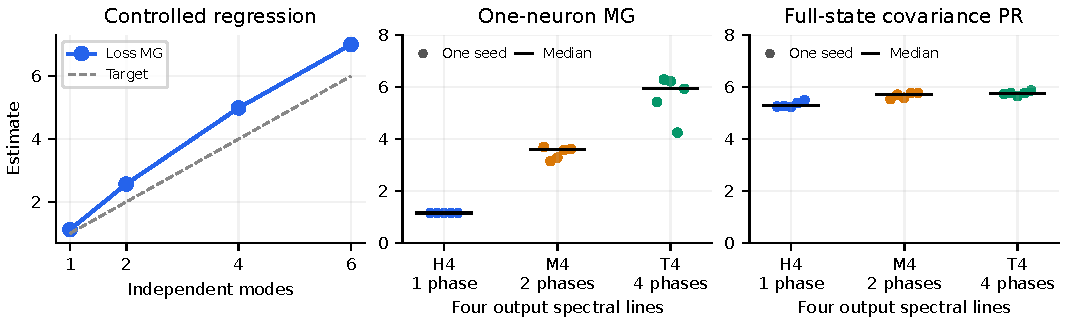
\includegraphics[width=.98\textwidth]{figures/components.pdf}
\caption{\claude{Phase structure recovered from scalar records. Left: regression with known modes; the dashed line is the target dimension. Center and right: generators with four output spectral lines and one (H4, blue), two (M4, orange), or four (T4, green) target phases. Dots represent seeds and black bars indicate medians. Single-neuron MG separates these phase structures despite similar full-state covariance participation ratios (PR).}}
\label{fig:components}
\end{figure*}

The harmonic comparison tests whether MG detects independent phases rather than spectral peaks (Figure~\ref{fig:components}, Table~\ref{tab:generator_phases}). For every seed, MG is lower for H2 than T2 and increases from H4 to M4 to T4. The latter tasks have identical numbers of spectral peaks and similar covariance PR. MG therefore distinguishes their phase structure from a single-neuron recording. It also separates T1 and T2 from the higher-dimensional tasks, but overestimates dimension for T3 and T4 and does not distinguish them at this record length.

\begin{table}[t]
\centering\small
\caption{\claude{Learned generator results: medians over five seeds. Phases denotes target dimension; MG uses neuron zero and PR uses the full state. For each seed, MG is the median over four 8,192-sample windows.}}
\label{tab:generator_phases}
\begin{tabular}{lrrr}
\toprule
Task & Phases & MG & Covariance PR \\
\midrule
T1 & 1 & 1.15 & 1.64 \\
T2 & 2 & 2.84 & 3.01 \\
T3 & 3 & 5.90 & 4.32 \\
T4 & 4 & 5.93 & 5.76 \\
H2 & 1 & 1.12 & 2.97 \\
H4 & 1 & 1.15 & 5.27 \\
M4 & 2 & 3.58 & 5.71 \\
\bottomrule
\end{tabular}

\end{table}

\subsection{FORCE training from chaos to periodic output}\label{sec:force}
In a separate FORCE experiment, a 256-unit network learns to produce a figure-eight trajectory from initially chaotic activity. The target has two outputs but one fundamental phase. We select five chaotic initializations using a pretraining Lyapunov criterion, without inspecting MG, and evaluate the network at saved checkpoints.

Single-neuron MG falls from 3.56--5.07 before training to 1.08--1.13 afterward in all five networks. The decline persists across three neurons and the tested window and lag settings. Independently, the full Lyapunov spectrum loses its clearly positive exponents. Four networks meet the stricter stable-cycle criterion; the fifth has weak contraction transverse to the cycle.

Both analyses identify simplification of the learned activity. MG does so from one neuron, while the spectrum uses the full state and tangent dynamics. Section~\ref{sec:cost} compares their computational costs. Here the measured trajectory is network activity at fixed weights, not the sequence of weight updates.
}
